\chapter{Clasificación con descriptor LBP Uniforme}
En este apartado se describirá la implementación de la clase \textit{ULBP}, que implementa el funcionamiento del descriptor LBP-Uniforme. Tras esto se mostrarán los resultados obtenidos por los descriptores generados por dicha clase y se analizarán y comparán con los obtenidos por los descriptores de los apartados anteriores. La implementación de la clase descrita y las pruebas realizadas se pueden encontrar en los ficheros \textbf{uniform\_lbp.py} y \textbf{prueba\_lbp\_uniforme.py}.

\section{Implementación del descriptor ULBP}
Para implementación de este descriptor se ha utilizado la clase \textit{LBP} del apartado anterior añadiendo funciones para obtener los códigos que genera LBP-Uniforme y modificando la función \textit{computeLBPpixel()} para que devuelva la etiqueta necesaria para dicho píxel en vez del valor que genera LBP de forma normal, para ello se ha implementado el método \textit{codeToLabel()}, dicha función tiene como argumento el código LBP generado en ese píxel (vector de 0s y 1s obtenido por la comparación del píxel con sus vecinos), la función devuelve la etiqueta de dicho código (que coincide con la posición en la que son generados los códigos uniformes), si no lo encuentra devuelve la etiqueta utilizada para códigos no uniformes (para el caso de 8 vecinos por píxel es 59).\\

Para no tener que calcular todos los códigos de LBP que son uniformes cada vez que se computa un descriptor, estos valores se calculan una vez se crea un objeto de la clase \textit{ULBP}. Para calcular estos valores se han implementado tres funciones nuevas. La función \textit{generateAllRotations()}, que tiene como argumentos el número de unos que tiene que haber dentro del código y el número, de esta forma, genera $numerodevecinos-1$ rotaciones del un código inicial; este código inicial es un vector con el número de unos indicado como argumento al principio y el resto ceros hasta completar el tamaño del código, esto lo hace la función \textit{generateInitialVec()}; para hacer una rotación se utiliza la función \textit{np.roll()} de la librería \textbf{numpy} que desplaza los elementos de un vector dado un número x de veces indicado. Una vez generadas todas las rotaciones, se devuelve un vector que las contiene. Por último se ha implementado \textit{generaUniformVects()} que tiene como argumentos el número de vecinos; esta función hace uso de las anteriores para generar todo el conjunto de códigos uniformes de LBP dado el número de vecinos para un píxel.

\begin{figure}[H]
	\centering
	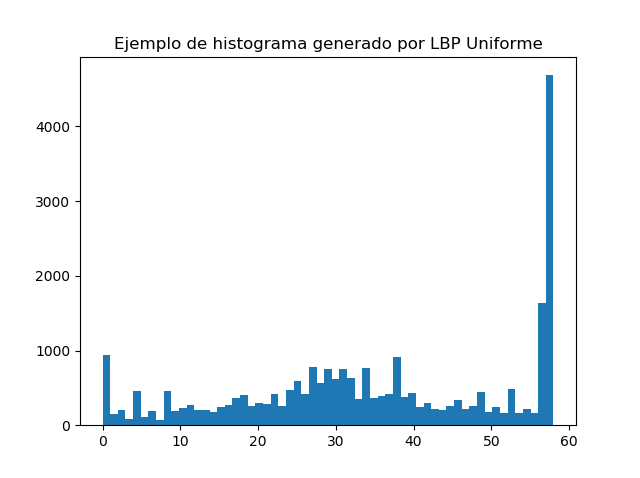
\includegraphics[width=140mm]{imagenes/ulbp_histogram}
	\caption{Ejemplo Histograma de un descriptor LBP}
	\label{fig:salida_4}
\end{figure}

\section{Pruebas con LBP Uniforme}
En esta sección se muestran los resultados obtenidos por modelos generados con los datos generados por el descriptor LBP-Uniforme. Los resultados son los siguientes: \\

\begin{table}[H]
	\begin{tabular}{llllll}
		\textbf{Validation} & \textbf{F1} & \textbf{accuracy} & \textbf{precision} & \textbf{truenegativerate} & \textbf{truepositiverate} \\
		0                   & 0.865234    & 0.872458          & 0.848659           & 0.863793                  & 0.882470                  \\
		1                   & 0.872093    & 0.878004          & 0.837989           & 0.851789                  & 0.909091                  \\
		2                   & 0.844534    & 0.856747          & 0.788390           & 0.817447                  & 0.909287                  \\
		3                   & 0.867133    & 0.877079          & 0.841085           & 0.862647                  & 0.894845                  \\
		4                   & 0.859556    & 0.877079          & 0.856842           & 0.888525                  & 0.862288                 
	\end{tabular}
	\caption{Validación con SVM kernel lineal}
	\label{table_19}
\end{table}

\begin{table}[H]
	\begin{tabular}{llllll}
		\textbf{Validation} & \textbf{F1} & \textbf{accuracy} & \textbf{precision} & \textbf{truenegativerate} & \textbf{truepositiverate} \\
		0                   & 0.642812    & 0.474122          & 0.473636           & 0.001754                  & 1.0                       \\
		1                   & 0.629512    & 0.459335          & 0.459335           & 0.000000                  & 1.0                       \\
		2                   & 0.618135    & 0.447320          & 0.447320           & 0.000000                  & 1.0                       \\
		3                   & 0.589693    & 0.418669          & 0.418131           & 0.001587                  & 1.0                       \\
		4                   & 0.614001    & 0.444547          & 0.443003           & 0.004967                  & 1.0                      
	\end{tabular}
	\caption{Validación con SVM kernel RBF}
	\label{table_20}
\end{table}

\begin{table}[H]
	\begin{tabular}{llllll}
		\textbf{Validation} & \textbf{F1} & \textbf{accuracy} & \textbf{precision} & \textbf{truenegativerate} & \textbf{truepositiverate} \\
		0                   & 0.865385    & 0.870610          & 0.830258           & 0.842466                  & 0.903614                  \\
		1                   & 0.877953    & 0.885397          & 0.851145           & 0.867797                  & 0.906504                  \\
		2                   & 0.870010    & 0.882625          & 0.853414           & 0.878939                  & 0.887265                  \\
		3                   & 0.869295    & 0.883549          & 0.846465           & 0.876020                  & 0.893390                  \\
		4                   & 0.848849    & 0.860444          & 0.820116           & 0.845000                  & 0.879668                 
	\end{tabular}
	\caption{Validación con SVM kernel polinómico grado 2}
	\label{table_21}
\end{table}

\begin{table}[H]
	\begin{tabular}{llllll}
		\textbf{Validation} & \textbf{F1} & \textbf{accuracy} & \textbf{precision} & \textbf{truenegativerate} & \textbf{truepositiverate} \\
		0                   & 0.870293    & 0.885397          & 0.845528           & 0.877023                  & 0.896552                  \\
		1                   & 0.882061    & 0.890018          & 0.854127           & 0.872054                  & 0.911885                  \\
		2                   & 0.877228    & 0.885397          & 0.847036           & 0.865546                  & 0.909651                  \\
		3                   & 0.862000    & 0.872458          & 0.850099           & 0.870968                  & 0.874239                  \\
		4                   & 0.864097    & 0.876155          & 0.827184           & 0.854337                  & 0.904459                 
	\end{tabular}
	\caption{Validación con SVM kernel polinómico grado 3}
	\label{table_22}
\end{table}

\begin{table}[H]
	\begin{tabular}{llllll}
		\textbf{Validation} & \textbf{F1} & \textbf{accuracy} & \textbf{precision} & \textbf{truenegativerate} & \textbf{truepositiverate} \\
		0                   & 0.869059    & 0.875231          & 0.820513           & 0.835846                  & 0.923711                  \\
		1                   & 0.883813    & 0.891867          & 0.849237           & 0.868114                  & 0.921325                  \\
		2                   & 0.859330    & 0.864140          & 0.825368           & 0.836489                  & 0.896208                  \\
		3                   & 0.875764    & 0.887246          & 0.838207           & 0.864600                  & 0.916844                  \\
		4                   & 0.847695    & 0.859519          & 0.804183           & 0.831148                  & 0.896186                 
	\end{tabular}
	\caption{Validación con SVM kernel polinómico grado 4}
	\label{table_23}
\end{table}

\begin{table}[H]
	\begin{tabular}{llllll}
		\textbf{Validation} & \textbf{F1} & \textbf{accuracy} & \textbf{precision} & \textbf{truenegativerate} & \textbf{truepositiverate} \\
		0                   & 0.627774    & 0.457486          & 0.457486           & 0.0                       & 1.0                       \\
		1                   & 0.621656    & 0.451017          & 0.451017           & 0.0                       & 1.0                       \\
		2                   & 0.616368    & 0.445471          & 0.445471           & 0.0                       & 1.0                       \\
		3                   & 0.619898    & 0.449168          & 0.449168           & 0.0                       & 1.0                       \\
		4                   & 0.619898    & 0.449168          & 0.449168           & 0.0                       & 1.0                      
	\end{tabular}
	\caption{Validación con SVM kernel polinómico grado 5}
	\label{table_24}
\end{table}

\begin{table}[H]
	\begin{tabular}{llllll}
		\textbf{Validation} & \textbf{F1} & \textbf{accuracy} & \textbf{precision} & \textbf{truenegativerate} & \textbf{truepositiverate} \\
		0                   & 0.640704    & 0.471349          & 0.471349           & 0.0                       & 1.0                       \\
		1                   & 0.644110    & 0.475046          & 0.475046           & 0.0                       & 1.0                       \\
		2                   & 0.592062    & 0.420518          & 0.420518           & 0.0                       & 1.0                       \\
		3                   & 0.643260    & 0.474122          & 0.474122           & 0.0                       & 1.0                       \\
		4                   & 0.602067    & 0.430684          & 0.430684           & 0.0                       & 1.0                      
	\end{tabular}
	\caption{Validación con SVM kernel sigmoidal}
	\label{table_25}
\end{table}

\begin{table}[H]
	\begin{tabular}{llllll}
		\textbf{Validation} & \textbf{F1} & \textbf{accuracy} & \textbf{precision} & \textbf{truenegativerate} & \textbf{truepositiverate} \\
		0                   & 0.621173    & 0.451017          & 0.450509           & 0.001681                  & 1.0                       \\
		1                   & 0.608360    & 0.437153          & 0.437153           & 0.000000                  & 1.0                       \\
		2                   & 0.618135    & 0.447320          & 0.447320           & 0.000000                  & 1.0                       \\
		3                   & 0.625556    & 0.455638          & 0.455134           & 0.001695                  & 1.0                       \\
		4                   & 0.625159    & 0.454713          & 0.454713           & 0.000000                  & 1.0                      
	\end{tabular}
	\caption{Validación con SVM kernel Chi Cuadrado}
	\label{table_26}
\end{table}

\begin{table}[H]
	\begin{tabular}{llllll}
		\textbf{Validation} & \textbf{F1} & \textbf{accuracy} & \textbf{precision} & \textbf{truenegativerate} & \textbf{truepositiverate} \\
		0                   & 0.924025    & 0.931608          & 0.912779           & 0.928453                  & 0.935551                  \\
		1                   & 0.928355    & 0.934381          & 0.918164           & 0.930743                  & 0.938776                  \\
		2                   & 0.937033    & 0.945471          & 0.940043           & 0.954248                  & 0.934043                  \\
		3                   & 0.938525    & 0.944547          & 0.952183           & 0.960818                  & 0.925253                  \\
		4                   & 0.922441    & 0.930684          & 0.915811           & 0.931894                  & 0.929167                 
	\end{tabular}
	\caption{Validación con SVM kernel Inter}
	\label{table_27}
\end{table}

Para este descriptor podemos observar que al igual que para el caso de LBP, obtenemos los mejores resultados con clasificador con kernel Inter, obteniendo resultados muy parecidos. Otros también ofrecen buenos resultados, como son los casos de los clasificadores con kernel lineal, polinómico de grado 2,3 y 4; para los que se pueden ver un rendimiento de entre un 85\% y un 90\% de acierto, superando además los resultados que se obtenían para LBP, esta diferencia puede ser provocada por la diferencia de rango entre ambos descriptores; para el caso de LBP tenemos 256 posibilidades diferentes de las cuales muchas de ellas no aportaban información realmente, para LBP-Uniforme tenemos (para los valores establecidos en esta práctica) 59 valores diferentes donde agrupamos todos los valores que aportaban poca información en uno solo; esto puede hacer que los clasificadores generalicen mejor y por ello obtengan mejores resultados. En el resto de clasificadores los resultados son parecidos a los que había en LBP, posiblemente estos estén provocados por el gran número de características de estos descriptores (26880) que hagan que los clasificadores no generalicen. \\

Aún habiendo mejorado los resultados conforme a LBP, el rendimiento de HOG sigue siendo superior al obtenido por LBP-Uniforme, habiendo una diferencia de entre 5-10\% en cada uno de los clasificadores. Esta diferencia aumenta para aquellos clasificadores que sobreajustan con LBP-Uniforme.  